%The default article class is limited to 12pt, but you can go up to 14, 17 or 20 points if you use the extarticle class:
\documentclass[a4paper,14pt]{extarticle}
\usepackage{cmap} %make LaTeX PDF output copy-and-pasteable
\usepackage[T2A]{fontenc}
\usepackage[utf8]{inputenc} %coding
\usepackage[english,ukrainian]{babel}
\usepackage{amssymb,amsfonts,amsmath,cite,enumerate,float}
\usepackage{indentfirst} %set an additional space before a paragraph at the begining of new section
\usepackage{graphicx}
\usepackage{wrapfig}
\usepackage{varwidth}
\usepackage{setspace}

\graphicspath{{images/}} %path to images

\usepackage[table,xcdraw]{xcolor}

\parskip=1mm %space between paragraphs

\usepackage{geometry} 
\geometry{left=1.25cm}
\geometry{right=1.25cm}
\geometry{top=1cm}
\geometry{bottom=2cm}

\usepackage{listings} %for code

\usepackage{color}

\definecolor{dkgreen}{rgb}{0,0.6,0}
\definecolor{gray}{rgb}{0.5,0.5,0.5}
\definecolor{mauve}{rgb}{0.58,0,0.82}

\lstset{
    frame=tb,
    language=Python,
    aboveskip=3mm,
    belowskip=3mm,
    showstringspaces=false,
    columns=flexible,
    basicstyle={\small\ttfamily},
    numbers=none,
    numberstyle=\tiny\color{gray},
    keywordstyle=\color{blue},
    commentstyle=\color{dkgreen},
    stringstyle=\color{mauve},
    breaklines=true,
    breakatwhitespace=true,
    tabsize=3
}

\begin{document}

\begin{titlepage}
    \newpage

    \begin{minipage}[c]{\linewidth}

        \newlength{\maxpreambula}
        \settowidth{\maxpreambula}{\small{<<Київський політехнічний інститут імені Ігоря Сікорського>>}}    

        \hspace{5cm}\parbox{\maxpreambula}{
            \begin{spacing}{1.1}\small{
                Міністерство освіти і науки України \\
                Національний технічний університет України \\
                <<Київський політехнічний інститут імені Ігоря Сікорського>> \\
                Навчально-науковий фізико-технічний інститут }
            \end{spacing}
        }
            
        \vspace*{-2.35cm}
        \hspace*{1.5cm}
        
\includegraphics[width=0.13\paperwidth]{kpi_emblem.png}

    \end{minipage}
    
    \vspace{\fill}
    
    \begin{center}
        \begin{spacing}{1.5}
            \textbf{\Large{Реалізація EM-алгоритму}} \\ 
            \vspace{1cm}\textbf{\normalsize{предмет <<Марковські моделі та їхнє застосування>>}}
        \end{spacing}
    \end{center}
    
    \vspace{\fill}
    
    \newlength{\maxname}
    \settowidth{\maxname}{\small{Цибульник Антон Владиславович}}

    \hfill\parbox{\maxname}{
        \begin{spacing}{1.1}
            \small{\textbf{Роботу виконав:}} \\ 
            \small{Студент групи ФІ-91,} \\
            \small{Цибульник Антон Владиславович} \\
        \end{spacing}
    }

    \hfill\parbox{\maxname}{
        \begin{spacing}{1.1}
            \small{\textbf{Роботу перевірила:}} \\ 
            \small{Ніщенко Ірина Іванівна} \\
        \end{spacing}
    }

    \vspace{0.5cm}

    \begin{center}
        \small{2022}
    \end{center}
    
\end{titlepage}

\newpage

\subsection*{Мета}
Ознайомитися з алгоритмом растрового подання відрізка.

\subsection*{Завдання} 
Написати програму, що реалізує алгоритм растрового малювання
відрізка.

\subsection*{Теоретичні відомості} 

У комп’ютерній графіці найбільш відомими є два типи візуалізації:
растровий та векторний. Перший спосіб асоціюється з такими графічними
пристроями, як дисплей, телевізор, принтер. Другий – для векторних
дисплеїв, плотерів. Оскільки пристроїв першого типу значно більше, то
частіше використовується растрова візуалізація зображень.

Растрова візуалізація ґрунтується на поданні зображення на екрані або
папері у вигляді сукупності окремих точок (пікселів). Разом піксели
утворюють растр. Таким чином, растр – це прямокутна матриця комірок
(пікселів). Кожен піксел має свій колір. Сукупність пікселів утворює
зображення.

\subsection*{Код програми}

\lstinputlisting[language=Python]{cg1.py}

\subsection*{Скріншоти результатів}

\begin{figure}[h]
    \begin{minipage}[h]{0.31\linewidth}
        \center{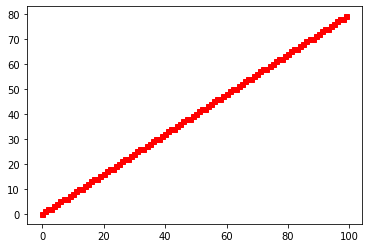
\includegraphics[width=1\linewidth]{line1.png}}
        \caption{red line}
    \end{minipage}
    \hfill
    \begin{minipage}[h]{0.31\linewidth}
        \center{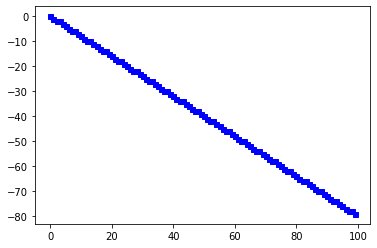
\includegraphics[width=1\linewidth]{line2.png}}
        \caption{blue line}
    \end{minipage}
    \hfill
    \begin{minipage}[h]{0.31\linewidth}
        \center{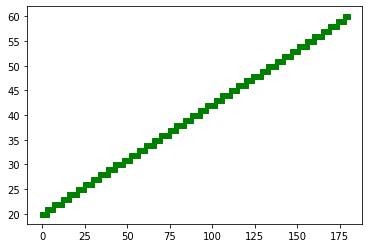
\includegraphics[width=1\linewidth]{line3.png}}
        \caption{green line}
    \end{minipage}
\end{figure}

\subsection*{Висновки}

У лабораторному практикумі я навчився будувати прямі методом 
цифрового диференціального аналізатора. Здобув практичні навички 
кодування алгоритму на мові python. Розглянув декілька варіантів побудови 
прямих в залежності відповідні заданих початкових та кінцевих точок.

\subsection*{Контрольні питання}

\begin{enumerate}

    \item Що називається розкладенням в растр?

    Процес визначення пікселів, найкращим чином апроксимуючих 
    заданий відрізок до елементів растру, називається 
    розкладенням в растр.

    \item Яка причина використання растеризації?

    У комп’ютерній графіці найбільш відомими є два типи 
    візуалізації: растровий та векторний. Перший спосіб 
    асоціюється з такими графічними пристроями, як дисплей, 
    телевізор, принтер. Другий – для векторних дисплеїв, 
    плотерів. Оскільки пристроїв першого типу значно більше, то 
    частіше використовується растрова візуалізація зображень.

    Оскільки екран електронно-променевої трубки можна розглядати 
    як матрицю дискретних елементів (пікселів), кожний з яких 
    може бути підсвічений, неможливо безпосередньо провести 
    відрізок із однієї точки в іншу. Саме тому використовують 
    процес растерізації - визначення прийнятних розміщень 
    замальованих пікселів.

    \item Опишіть ідею, що покладена в основу алгоритму цифрового 
    диференціального аналізатора.

    Ідея полягає в тому, щоб на кожній ітерації порівнювати 
    відстань від прямої до можливих пікселів, тобто 
    значень-претендентів. Яка відстань менша - ближчий піксель 
    і замальовуємо.

\end{enumerate}

\end{document}